\documentclass[a4paper]{article}

\usepackage{verbatim}
\usepackage{tikz}
\usetikzlibrary{calc, external, intersections, through}
\tikzexternalize[prefix=tikz/]

\textwidth=15cm
\textheight=23cm
\topmargin=0pt
\headheight=0pt
\oddsidemargin=2em
\headsep=0pt
\parindent=0pt

\begin{document}
\thispagestyle{empty}

\begin{center}
\textbf{\sffamily \Large Visualization of Theorems of Geometry}

\bigskip

\textbf{\sffamily \large Moti Ben-Ari}

\bigskip

\textbf{\sffamily \large http://www.weizmann.ac.il/sci-tea/benari/}

\end{center}

\textsf{\footnotesize \copyright{} 2017 by Moti Ben-Ari. This work is licensed under the Creative Commons Attribution-ShareAlike 3.0 Unported License. To view a copy of this license, visit http://creativecommons.org/licenses/by-sa/3.0/ or send a letter to Creative Commons, 444 Castro Street, Suite 900, Mountain View, California, 94041, USA.}

\bigskip

%%%%%%%%%%%%%%%%%%%%%%%%%%% First page %%%%%%%%%%%%%%%%%%%%%%%%%%%%%%

%% Pair 1

% Inscribed circle center at meeting of angle bisectors
%
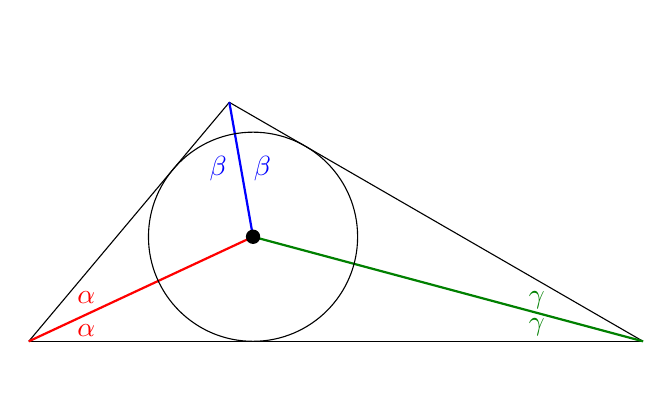
\begin{tikzpicture}[baseline=-6mm,scale=1.3]
% Draw base and path two lines at known angles
\draw (0,0) coordinate (a) -- (0:6) coordinate (b);
\path[name path=ac] (a) -- +(50:4);
\path[name path=bc] (b) -- +(150:5);
% Get their intersection and draw lines to third vertex
\path[name intersections={of=ac and bc,by=c}];
\draw (a) -- (c) -- (b);
% Path bisectors of two lines
\path[name path=bia,blue] (a) -- +(25:3.5);
\path[name path=bib,red] (b) -- +(165:5);
% Intersection of angle bisectors
\path [name intersections={of=bia and bib,by=center}];
% Draw angle bisectors to center
\draw[thick,red] (a) -- (center);
\draw[thick,blue] (c) -- (center);
\draw[thick,green!50!black] (b) -- (center);
% Labels of angles
\node[red,right,xshift=14pt,yshift=4pt] at (a) {$\alpha$};
\node[red,right,xshift=14pt,yshift=16pt] at (a) {$\alpha$};
\node[blue,below,xshift=-4pt,yshift=-16pt] at (c) {$\beta$};
\node[blue,below,xshift=12pt,yshift=-16pt] at (c) {$\beta$};
\node[green!50!black,left,xshift=-32pt,yshift=5pt] at (b) {$\gamma$};
\node[green!50!black,left,xshift=-32pt,yshift=15pt] at (b) {$\gamma$};
% Get perpendicular from center to one side and draw circle
\coordinate (perp) at ($(a)!(center)!(b)$);
\node [draw,circle through=(perp)] at (center) {};
% Draw dot at center
\fill (center) circle (2pt);
\end{tikzpicture}
%
\hspace{\fill}
%
% Perpendicular bisectors meet in the center of the circumscribed circle
%
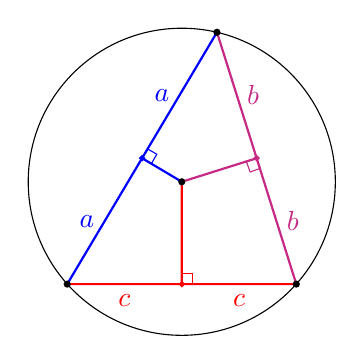
\begin{tikzpicture}[scale=.65]
% Circle goes from (a) to (b)
\coordinate (a) at (0,0);
\coordinate (b) at (6,0);
% Line containing lower points is (c) -- (d)
\coordinate (c) at (0,-2);
\coordinate (d) at (6,-2);
% Line containing upper points is (e) -- (f)
\coordinate (e) at (0,2);
\coordinate (f) at (4,3);
% Name the two chords
\path [name path=chord1] (c) -- (d);
\path [name path=chord2] (e) -- (f);
% Name the coordinate of the center of the circle
\coordinate (center) at ($ (a)!.5!(b) $);
% Draw a circle whose center is half-way between (a) and (b) through (a)
\node [draw,circle through=(a),name path=circ] at (center) {};
% Get intersections of the upper and lower lines with the circle
\path [name intersections={of=circ and chord1,by={i1,i2}}];
\path [name intersections={of=circ and chord2,by={i3,i4}}];
% Draw triangle
\draw [thick,blue] (i1) -- node[left] {$a$} ($(i1)!.5!(i3)$) --
  node[left] {$a$} (i3);
\draw[thick,magenta!80!black] (i3) -- node[right] {$b$} ($(i3)!.5!(i2)$) --
  node[right] {$b$} (i2);
\draw[thick,red] (i2) -- node[below] {$c$} ($(i2)!.5!(i1)$) -- 
  node[below] {$c$} (i1);
% Draw three perpendicular bisectors
\draw [thick,red,fill] (center) -- ($(i1)!(center)!(i2)$)
  circle[radius=1pt];
\draw [thick,blue,fill] (center) -- ($(i1)!(center)!(i3)$)
  circle[radius=1pt];
\draw [thick,magenta!80!black,fill] (center) -- ($(i2)!(center)!(i3)$)
  circle[radius=1pt];
% Draw squares to denote right angles
\draw[red] ($ (i1) !.5! (i2) $) rectangle +(6pt,6pt);
\draw[blue,rotate=-30] ($ (i1) !.5! (i3) $) rectangle +(6pt,6pt);
\draw[magenta!80!black,rotate=-160] ($ (i3) !.5! (i2) $)
  rectangle +(6pt,6pt);
% Draw dots at all intersections
\fill (i1) circle (2pt);
\fill (i2) circle (2pt);
\fill (i3) circle (2pt);
\fill (center) circle (2pt);
\end{tikzpicture}

%% Pair 2

\bigskip
\bigskip

% Angles of tangent and angle subtending a chord are equal
%
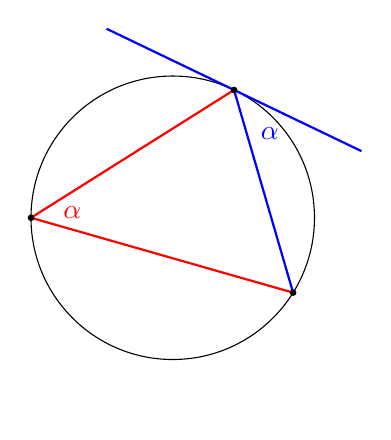
\begin{tikzpicture}[scale=.6,baseline=-70pt]
% Circle goes from (a) to (b)
\coordinate (a) at (0,0);
\coordinate (b) at (6,0);
% Line containing lower point (d)
\coordinate (d) at (7,-2);
% Point outside circle is (e)
\coordinate (e) at (1.6,4);
% Name the lower chord
\path [name path=chord] (a) -- (d);
% Draw a circle whose center is half-way between (a) and (b) through (a)
\node [draw,circle through=(a),name path=circ] (circle) at ($ (a)!.5!(b) $) {};
% Get intersection of the lower line with the circle
\path [name intersections={of=circ and chord,by={i1,i2}}];
% Draw the tangent line
\coordinate (tan) at (tangent cs:node=circle, point={(e)}, solution=2);
\draw[thick,blue] (e) -- ($ (e)!2!(tan) $);
% Draw the triangle
\draw [thick,blue] (tan) node[below right,xshift=6pt,yshift=-10pt] {$\alpha$} -- (i2);
\draw [thick,red] (tan) -- (a) node[right,xshift=8pt,yshift=2pt] {$\alpha$} -- (i2);
% Dots at intersections
\fill (a) circle (2pt);
\fill (i2) circle (2pt);
\fill (tan) circle(2pt);
\end{tikzpicture}
%
\hspace{\fill}
%
% Intersecting secants
%
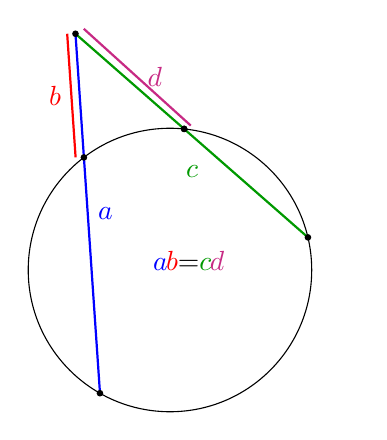
\begin{tikzpicture}[scale=.6]
% Circle goes from (a) to (b)
\coordinate (a) at (0,0);
\coordinate (b) at (6,0);
% Line containing lower points is (c) -- (d)
\coordinate (c) at (1,-3);
\coordinate (d) at (7,1.5);
% Point outside circle is (e)
\coordinate (e) at (1,5);
% Name the lower chord
\path [name path=chord] (c) -- (d);
% Draw a circle whose center is half-way between (a) and (b) through (a)
\node [draw,circle through=(a),name path=circ] at ($ (a)!.5!(b) $) {};
% Get intersection of the lower line with the circle
\path [name intersections={of=circ and chord,by={i1,i2}}];
% Draw the full secants
\draw [name path=secant1,thick,green!60!black] (i1) -- node[left,xshift=6pt,yshift=-13pt] {$c$} (e);
\draw [name path=secant2,thick,blue] (i2) -- node[right] {$a$} (e);
% Get intersections of the secants with the circle
\path [name intersections={of=circ and secant1,by={s11,s12}}];
\path [name intersections={of=circ and secant2,by={s21,s22}}];
% Draw offset lines from outside point with the intersections of the secants
\draw[thick,red]
  let \p1 = (s21), \p2 = (e) in
    (\x2-5pt,\y2) -- node[left] {$b$} (\x1-5pt,\y1);
\draw[thick,magenta!80!black]
  let \p1 = (s12), \p2 = (e) in
    (\x2+5pt,\y2+3pt) -- node[right] {$d$} (\x1+4pt,\y1+2pt);
% Dots at intersections
\fill (s11) circle (2pt);
\fill (s12) circle (2pt);
\fill (s21) circle (2pt);
\fill (s22) circle (2pt);
\fill (s12) circle (2pt);
\fill (e) circle (2pt);
% Display formula in color
\begin{scope}[xshift=2.8cm]
\node[anchor=base,blue] at (0,0) {$a$};
\node[anchor=base,red] at (7pt,0) {$b$};
\node[anchor=base] at (17pt,0) {$=$};
\node[anchor=base,green!60!black] at (27pt,0) {$c$};
\node[anchor=base,magenta!80!black] at (34pt,0) {$d$};
\end{scope}
\end{tikzpicture}

\bigskip
\bigskip

%% Pair 3

% Medians of a triangle meet at a point with ratio 1:2
%
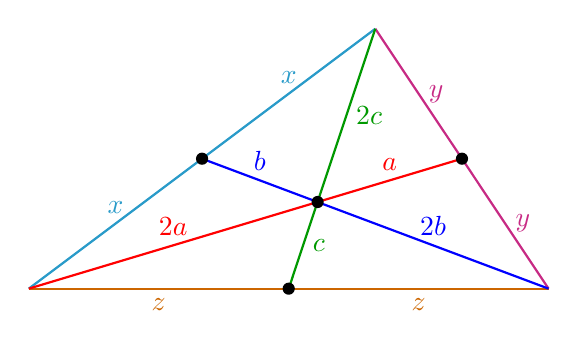
\begin{tikzpicture}[scale=1.1]
\coordinate (a) at (0,0);   % Points of the triangle
\coordinate (b) at (6,0);
\coordinate (c) at (4,3);
% Coordinates of bisectors
\coordinate (ab) at ($(a)!.5!(b)$);
\coordinate (bc) at ($(b)!.5!(c)$);
\coordinate (ac) at ($(a)!.5!(c)$);
% Draw the triangle and bisectors
\draw[cyan!80!black,thick] (a) -- node[above] {$x$} (ac) -- node[above] {$x$} (c);
\draw[magenta!80!black,thick] (b) -- node[right] {$y$} (bc) -- node[right] {$y$} (c);
\draw[orange!80!black,thick] (a) -- node[below] {$z$} (ab) -- node[below] {$z$} (b);
\draw[thick,red,name path=da] (a) -- (bc);
\draw[thick,blue,name path=db] (b) -- (ac);
\draw[thick,green!60!black,name path=dc] (c) -- (ab);
% Get their intersection
\path [name intersections={of=da and db,by={intersection}}];
% Labels
\path (a) -- node[above,red] {$2a$} (intersection);
\path (bc) -- node[above,red] {$a$} (intersection);
\path (b) -- node[above,blue] {$2b$} (intersection);
\path (ac) -- node[above,blue] {$b$} (intersection);
\path (c) -- node[right,green!60!black] {$2c$} (intersection);
\path (ab) -- node[right,green!60!black] {$c$} (intersection);
% Points at the intersections
\fill (intersection) circle (2pt);
\fill (ab) circle (2pt);
\fill (ac) circle (2pt);
\fill (bc) circle (2pt);
\end{tikzpicture}
%
\hspace{\fill}
%
% Angle bisector splits opposite side at same ratio as sides
%
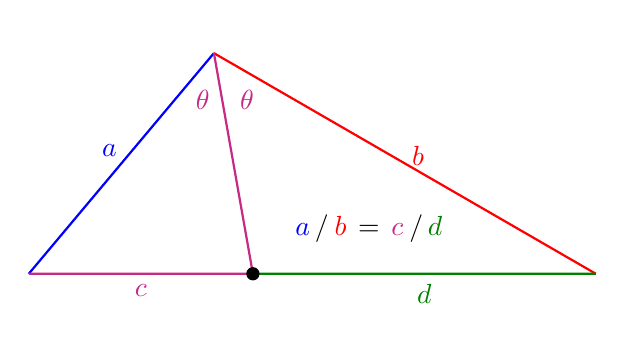
\begin{tikzpicture}[baseline=-4mm,scale=1.2]
% Draw base and path two lines at known angles
\path[name path=ab] (0,0) coordinate (a) -- (0:6) coordinate (b);
\path[name path=ac] (a) -- node[left,xshift=-2pt,blue] {$a$} +(50:3.4);
\path[name path=bc] (b) -- node[right,xshift=4pt,red] {$b$} +(150:5);
% Get their intersection and draw lines to third vertex
\path[name intersections={of=ac and bc,by=c}];
\draw[blue,thick] (a) -- (c);
\draw[red,thick] (c) -- (b);
% Path bisectors of two lines
\path[name path=bisector] (c) -- +(-80:2.5);
% Intersection of angle bisectors
\path [name intersections={of=bisector and ab,by=int}];
% Draw base of triangle
\draw[thick,magenta!80!black] (a) -- node[below] {$c$} (int);
\draw[thick,green!50!black] (int) -- node[below] {$d$} (b);
% Draw bisector and label angle
\draw[magenta!80!black,thick] (c) -- (int);
\node[magenta!80!black,below,xshift=-4pt,yshift=-10pt] at (c) {$\theta$};
\node[magenta!80!black,below,xshift=12pt,yshift=-10pt] at (c) {$\theta$};
 Draw dot
\fill (int) circle (2pt);
% Display formula in color
\begin{scope}[xshift=29mm,yshift=4mm]
\node[anchor=base,blue] at (0,0) {$a$};
\node[anchor=base] at (.2,0) {$/$};
\node[anchor=base,red] at (.4,0) {$b$};
\node[anchor=base] at (.7,0) {$=$};
\node[anchor=base,magenta!80!black] at (1,0) {$c$};
\node[anchor=base] at (1.2,0) {$/$};
\node[anchor=base,green!50!black] at (1.4,0) {$d$};
\end{scope}
\end{tikzpicture}

%% Pair 4


\bigskip
\bigskip

% Thale's theorem 2
%
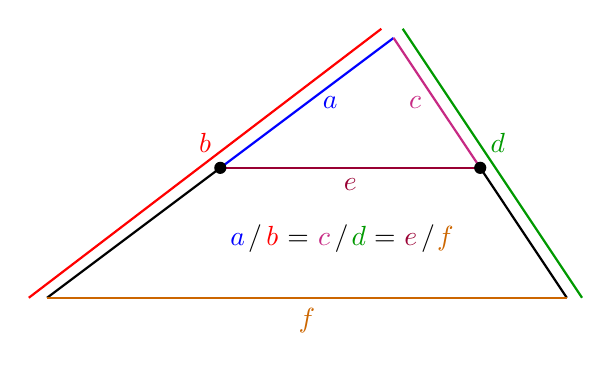
\begin{tikzpicture}[scale=1.1]
% Points of the triangle
\coordinate (a) at (0,0);
\coordinate (b) at (6,0);
\coordinate (c) at (4,3);
% Midpoints of the sides
\coordinate (mid1) at ($(a)!.5!(c)$);
\coordinate (mid2) at ($(b)!.5!(c)$);
% Midpoint of the base
\coordinate (midbase) at ($(a)!.5!(b)$);
\draw[thick] (a) -- (mid1);
\draw[thick,blue] (mid1) -- node[right,xshift=2pt] {$a$} (c);
\draw[thick] (b) -- (mid2);
\draw[thick,magenta!80!black] (mid2) -- node[left,xshift=-2pt] {$c$} (c);
% Draw the offest lines
\draw[thick,red]
  let \p1 = (a), \p2 = (c) in
    (\x1-6pt,\y1) -- node[above] {$b$} (\x2-4pt,\y2+3pt);
\draw[thick,green!60!black]
  let \p1 = (b), \p2 = (c) in
    (\x1+5pt,\y1) -- node[above,xshift=2pt] {$d$} (\x2+3pt,\y2+3pt);
% Draw the base and median
\draw[thick,orange!80!black] (a) -- node[below] {$f$} (b);
\draw[thick,purple!80!black] (mid1) -- node[below] {$e$} (mid2);
% Points at the midpoints
\fill (mid1) circle (2pt);
\fill (mid2) circle (2pt);
% Display formula in color
\begin{scope}[xshift=2.2cm,yshift=.6cm]
\node[anchor=base,blue] at (0,0) {$a$};
\node[anchor=base] at (.2,0) {$/$};
\node[anchor=base,red] at (.4,0) {$b$};
\node[anchor=base] at (.7,0) {$=$};
\node[anchor=base,magenta!80!black] at (1,0) {$c$};
\node[anchor=base] at (1.2,0) {$/$};
\node[anchor=base,green!60!black] at (1.4,0) {$d$};
\node[anchor=base] at (1.7,0) {$=$};
\node[anchor=base,purple!80!black] at (2,0) {$e$};
\node[anchor=base] at (2.2,0) {$/$};
\node[anchor=base,orange!80!black] at (2.4,0) {$f$};
\end{scope}
\end{tikzpicture}
%
\hspace{\fill}
% Median of a triangle is half the base
%
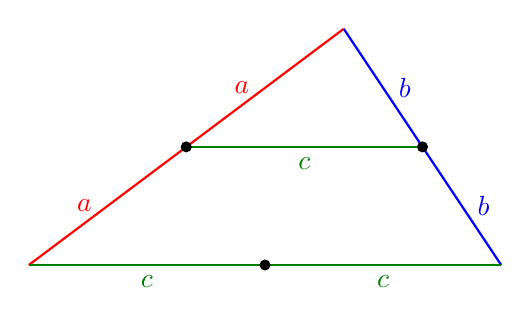
\begin{tikzpicture}
% Points of the triangle
\coordinate (a) at (0,0);
\coordinate (b) at (6,0);
\coordinate (c) at (4,3);
% Midpoints of the sides
\coordinate (mid1) at ($(a)!.5!(c)$);
\coordinate (mid2) at ($(b)!.5!(c)$);
% Midpoint of the base
\coordinate (midbase) at ($(a)!.5!(b)$);
% Draw the sides of the triangle: the base is drawn in two parts
\draw[thick,red] (a) -- node[left,xshift=-2pt] {$a$} (mid1);
\draw[thick,red] (mid1) -- node[left,xshift=-2pt] {$a$} (c);
\draw[thick,blue] (b) -- node[right,xshift=2pt] {$b$} (mid2);
\draw[thick,blue] (mid2) -- node[right,xshift=2pt] {$b$} (c);
% Draw the median
\draw[thick,green!50!black] (mid1) -- node[below] {$c$} (mid2);
% Draw the base
\draw[thick,green!50!black] (a) -- node[below] {$c$} (midbase);
\draw[thick,green!50!black] (b) -- node[below] {$c$} (midbase);
% Draw dots at the midpoints
\fill (mid1) circle (2pt);
\fill (mid2) circle (2pt);
\fill (midbase) circle (2pt);
\end{tikzpicture}

%%%%%%%%%%%%%%%%%%%%%%%%%%% Second page %%%%%%%%%%%%%%%%%%%%%%%%%%%%%%

\newpage

\thispagestyle{empty}

%% Pair 1

% Bisector of the hypotenuse is half the hypotenuse
%
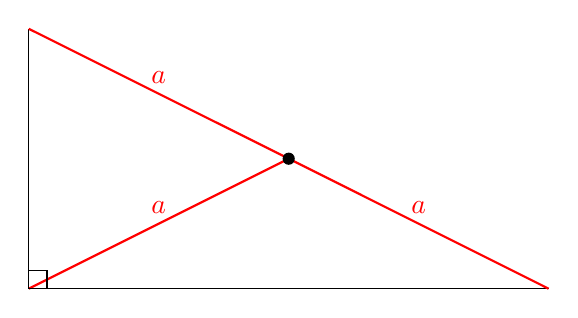
\begin{tikzpicture}[scale=1.1]
\coordinate (a) at (0,0);   % Points of the triangle
\coordinate (b) at (6,0);
\coordinate (c) at (0,3);
% Coordinate of bisector
\coordinate (hyp) at ($(b)!.5!(c)$);
% Draw the triangle and bisectors
\draw (b) -- (a) -- (c);
\draw[thick,red] (a) -- node[above,red] {$a$} (hyp);
\draw[thick,red] (b) -- node[above,red] {$a$} (hyp);
\draw[thick,red] (c) -- node[above,red] {$a$} (hyp);
% Draw square to denote right angle
\draw (a) rectangle +(6pt,6pt);
% Points at the intersections
\fill (hyp) circle (2pt);
\end{tikzpicture}
%
\hspace{\fill}
%
% Median of a trapeze is average of sides
%
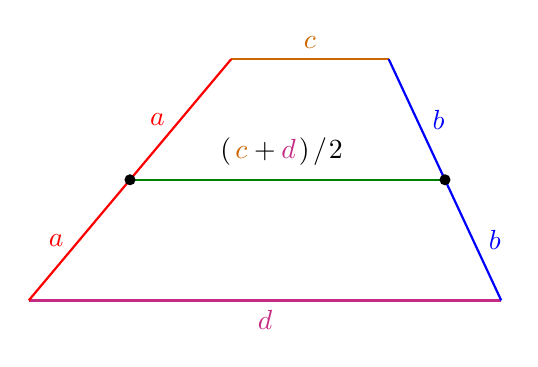
\begin{tikzpicture}
% Bottom of trapeze
\coordinate (a) at (0,0);
\coordinate (b) at (6,0);
% Draw the bases of the trapeze
\draw[thick,magenta!80!black] (a) -- node[below] {$d$} (b);
\path (a) -- ++(50:4) coordinate (c) -- ++(2,0) coordinate (d);
\draw[thick,orange!80!black] (c) -- node[above] {$c$} (d);
% Draw the sides of the trapeze in two parts
\coordinate (mid1) at ($(a)!.5!(c)$);
\coordinate (mid2) at ($(b)!.5!(d)$);
\draw[thick,red] (a) -- node[left,xshift=-2pt] {$a$} (mid1);
\draw[thick,red] (mid1) -- node[left,xshift=-2pt] {$a$} (c);
\draw[thick,blue] (b) -- node[right,xshift=2pt] {$b$} (mid2);
\draw[thick,blue] (mid2) -- node[right,xshift=2pt] {$b$} (d);
% Draw the median
\draw[thick,green!50!black] (mid1) -- (mid2);
% Display formula in color
\begin{scope}[xshift=25mm,yshift=18mm]
\node[anchor=base] at (0,0) {$($};
\node[anchor=base,orange!80!black] at (.2,0) {$c$};
\node[anchor=base] at (.5,0) {$+$};
\node[anchor=base,magenta!80!black] at (.8,0) {$d$};
\node[anchor=base] at (1.0,0) {$)$};
\node[anchor=base] at (1.2,0) {$/$};
\node[anchor=base] at (1.4,0) {$2$};
\end{scope}

% Dots at the midpoints
\fill (mid1) circle (2pt);
\fill (mid2) circle (2pt);
\end{tikzpicture}

%% Pair 2

\bigskip
\bigskip

% Diagonals of parallelogram bisect each other
%
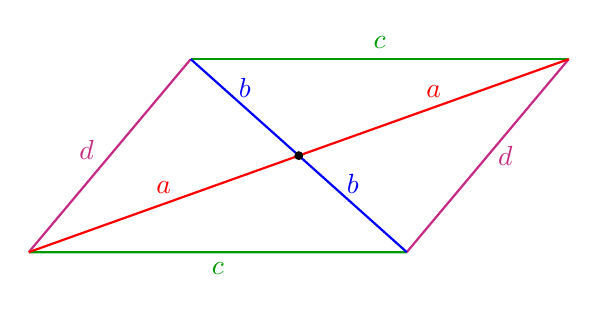
\begin{tikzpicture}[scale=.8]
% Bottom side of parallelogram
\coordinate (a) at (0,0);
\coordinate (b) at (6,0);
% Draw parallelogram at angle 50
\draw[thick,magenta!80!black] (a) -- node[left,xshift=-2pt,yshift=2pt] {$d$} +(50:4) coordinate (c);
\draw[thick,green!60!black] (c) -- node[above] {$c$} +(6,0) coordinate (d);
\draw[thick,magenta!80!black] (d) -- node[right] {$d$} +(230:4) coordinate (b);
\draw[thick,green!60!black] (b) -- node[below] {$c$} (a);
% Name the two diagonals
\path [name path=d1] (a) -- (d);
\path [name path=d2] (b) -- (c);
% Get their intersection
\path [name intersections={of=d1 and d2,by={intersection}}];
% Draw diagonals
\draw[thick,red] (a) -- node[above] {$a$} (intersection);
\draw[thick,red] (intersection) -- node[above] {$a$} (d);
\draw[thick,blue] (b) -- node[above] {$b$} (intersection);
\draw[thick,blue] (intersection) -- node[above] {$b$} (c);
% Dot at their intersection
\fill (intersection) circle (2pt);
\end{tikzpicture}
%
\hspace{\fill}
%
% Diagonals of rhombus bisect each other and are perpendicular
%
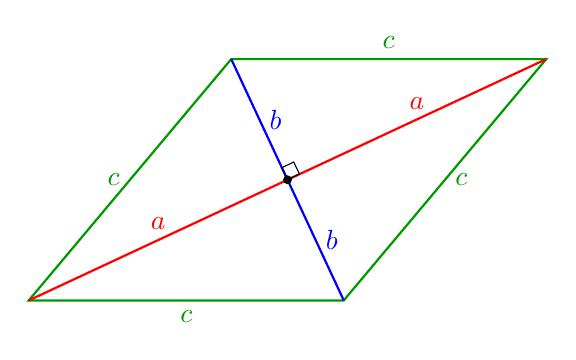
\begin{tikzpicture}[scale=.8]
% Bottom side of rhombus
\coordinate (a) at (0,0);
\coordinate (b) at (5,0);
% Draw rhombus at angle 50
\draw[thick,green!60!black] (a) -- node[left] {$c$} ++(50:5) coordinate (c) -- node[above] {$c$} ++(5,0) coordinate (d) -- node[right] {$c$} (b) -- node[below] {$c$} cycle;
% Name the two diagonals
\path [name path=d1] (a) -- (d);
\path [name path=d2] (b) -- (c);
% Get their intersection
\path [name intersections={of=d1 and d2,by={intersection}}];
% Draw diagonals
\draw[thick,red] (a) -- node[above] {$a$} (intersection);
\draw[thick,red] (intersection) -- node[above] {$a$} (d);
\draw[thick,blue] (b) -- node[right] {$b$} (intersection);
\draw[thick,blue] (intersection) -- node[right] {$b$} (c);
% Draw square to denote right angle
\draw[rotate=26] (intersection) rectangle +(6pt,6pt);
% Dot at their intersection
\fill (intersection) circle (2pt);
\end{tikzpicture}

%% Pair 3

\bigskip
\bigskip

%
% Sums of opposite sides of circumscribed quadrilateral are equal
%
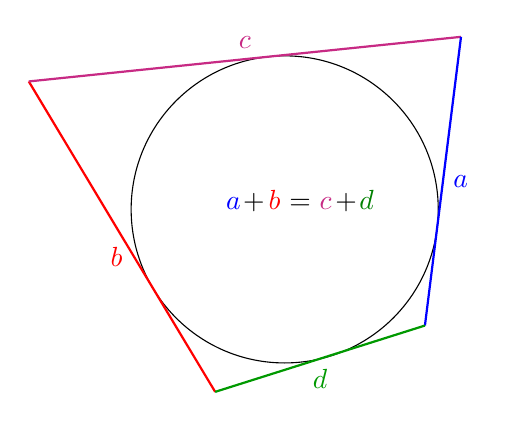
\begin{tikzpicture}[scale=.65]
% Circle goes from (a) to (b)
\coordinate (x) at (0,3);
\coordinate (y) at (6,3);
\coordinate (a) at (-2,5.5);
% Draw a circle whose center is half-way between (a) and (b) through (a)
\node [draw,circle through=(x),name path=circ] (circle) at ($ (x)!.5!(y) $) {};
% Draw tangent lines
\coordinate (tan1) at (tangent cs:node=circle, point={(a)}, solution=1);
\draw[thick,red] (a) -- node[below,xshift=-2pt] {$b$}
  ($(a)!1.5!(tan1)$) coordinate (b);
\coordinate (tan2) at (tangent cs:node=circle, point={(a)}, solution=2);
\draw[thick,magenta!80!black] (a) -- node[above] {$c$}
  ($(a)!1.8!(tan2)$) coordinate (c);
\coordinate (tan3) at (tangent cs:node=circle, point={(c)}, solution=2);
\draw[thick,blue] (c) -- node[right] {$a$}
  ($(c)!1.51!(tan3)$)  coordinate (d);
\draw[thick,green!60!black] (b) -- node[below] {$d$} (d);
% Display formula in color
\begin{scope}[xshift=2cm,yshift=3cm]
\node[anchor=base,blue] at (0,0) {$a$};
\node[anchor=base] at (.4,0) {$+$};
\node[anchor=base,red] at (.8,0) {$b$};
\node[anchor=base] at (1.3,0) {$=$};
\node[anchor=base,magenta!80!black] at (1.8,0) {$c$};
\node[anchor=base] at (2.2,0) {$+$};
\node[anchor=base,green!50!black] at (2.6,0) {$d$};
\end{scope}
\end{tikzpicture}
%
\hspace{\fill}
%
% Intersecting tangent and secant
%
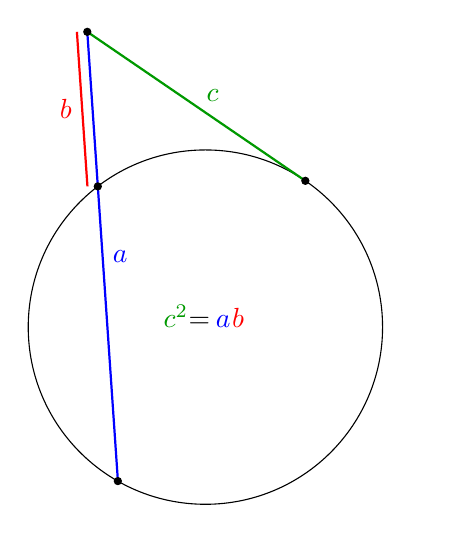
\begin{tikzpicture}[scale=.75]
% Circle goes from (a) to (b)
\coordinate (a) at (0,0);
\coordinate (b) at (6,0);
% Line containing lower points is (c) -- (d)
\coordinate (c) at (1,-3);
\coordinate (d) at (7,1.5);
% Point outside circle is (e)
\coordinate (e) at (1,5);
% Name the lower chord
\path [name path=chord] (c) -- (d);
% Draw a circle whose center is half-way between (a) and (b) through (a)
\node [draw,circle through=(a),name path=circ] (circle) at ($ (a)!.5!(b) $) {};
% Get intersection of the lower line with the circle
\path [name intersections={of=circ and chord,by={i1,i2}}];
% Draw the full secant
\draw [name path=secant2,thick,blue] (i2) -- node[right] {$a$} (e);
% Get intersection of the secant with the circle
\path [name intersections={of=circ and secant2,by={s21,s22}}];
% Draw offset line from outside point with the intersection of the secant
\draw[thick,red]
  let \p1 = (s21), \p2 = (e) in
    (\x2-5pt,\y2) -- node[left] {$b$} (\x1-5pt,\y1);
% Draw the tangent line
\coordinate (tan) at (tangent cs:node=circle, point={(e)}, solution=2);
\draw[thick,green!60!black] (e) -- node[right,yshift=4pt] {$c$} (tan);
% Dots at intersections
\fill (s21) circle (2pt);
\fill (s22) circle (2pt);
\fill (e) circle (2pt);
\fill (tan) circle(2pt);
% Display formula in color
\begin{scope}[xshift=2.5cm]
\node[anchor=base,green!60!black] at (0,0) {$c^2$};
\node[anchor=base] at (.4,0) {$=$};
\node[anchor=base,blue] at (.8,0) {$a$};
\node[anchor=base,red] at (30pt,0) {$b$};
\end{scope}
\end{tikzpicture}

%% Pair 4

\bigskip
\bigskip

%
% Opposite angles in an inscribed quadrilateral add up to 180
%
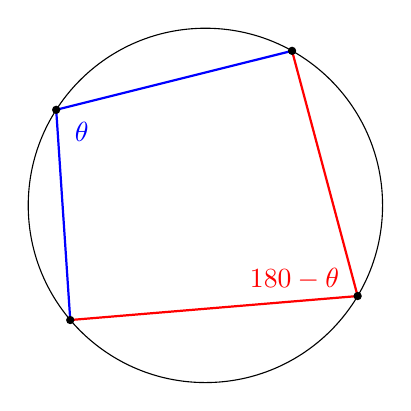
\begin{tikzpicture}[scale=.75]
% Circle goes from (a) to (b)
\coordinate (a) at (0,0);
\coordinate (b) at (6,0);
% Line containing lower points is (c) -- (d)
\coordinate (c) at (0,-2);
\coordinate (d) at (6,-1.5);
% Line containing upper points is (e) -- (f)
\coordinate (e) at (0,1.5);
\coordinate (f) at (6,3);
% Name the upper and lower lines
\path [name path=chord1] (c) -- (d);
\path [name path=chord2] (e) -- (f);
% Draw a circle whose center is half-way between (a) and (b) through (a)
\node [draw,circle through=(a),name path=circ] at ($ (a)!.5!(b) $) {};
% Get intersections of the upper and lower lines with the circle
\path [name intersections={of=circ and chord1,by={i1,i2}}];
\path [name intersections={of=circ and chord2,by={i3,i4}}];
% Draw the two subtended angles
\draw[thick,red] (i1) -- (i2)
  node[left,xshift=-3pt,yshift=6pt] {$180-\theta$} -- (i3);
\draw[thick,blue] (i1) -- (i4)
  node[right,xshift=3pt,yshift=-8pt] {$\theta$} -- (i3);
% Dots at intersections
\fill (i1) circle (2pt);
\fill (i2) circle (2pt);
\fill (i3) circle (2pt);
\fill (i4) circle (2pt);
\end{tikzpicture}
%
\hspace{\fill}
% Intersecting chords
%
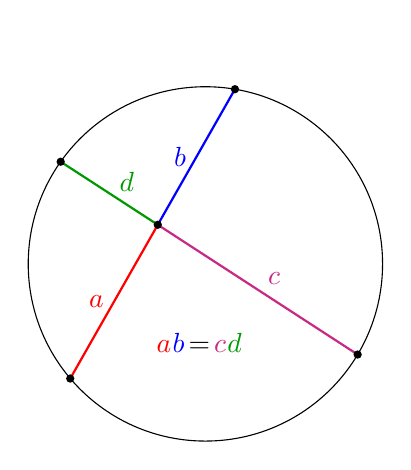
\begin{tikzpicture}[scale=.75]
% Circle goes from (a) to (b)
\coordinate (a) at (0,0);
\coordinate (b) at (6,0);
% Line containing lower points is (c) -- (d)
\coordinate (c) at (0,-2);
\coordinate (d) at (6,-1.5);
% Line containing upper points is (e) -- (f)
\coordinate (e) at (0,1.5);
\coordinate (f) at (6,4);
% Name the upper and lower lines
\path [name path=chord1] (c) -- (d);
\path [name path=chord2] (e) -- (f);
% Draw a circle whose center is half-way between (a) and (b) through (a)
\node [draw,circle through=(a),name path=circ] at ($ (a)!.5!(b) $) {};
% Get intersections of the upper and lower lines with the circle
\path [name intersections={of=circ and chord1,by={i1,i2}}];
\path [name intersections={of=circ and chord2,by={i3,i4}}];
% Name the two chords
\path [name path=x1] (i1) -- (i3);
\path [name path=x2] (i2) -- (i4);
% Get their intersection
\path [name intersections={of=x1 and x2,by={p}}];
% Draw four lines from intersection to circle
\draw[thick,red] (i1) -- node[left] {$a$} (p);
\draw[thick,blue] (p) --  node[left] {$b$} (i3);
\draw[thick,magenta!80!black] (i2) -- node[right,yshift=4pt] {$c$} (p);
\draw[thick,green!60!black] (p) -- node[right,yshift=4pt] {$d$} (i4);
% Dots at intersections
\fill (p) circle (2pt);
\fill (i1) circle (2pt);
\fill (i2) circle (2pt);
\fill (i3) circle (2pt);
\fill (i4) circle (2pt);
% Display formula in color
\begin{scope}[xshift=2.3cm,yshift=-1.5cm]
\node[anchor=base,red] at (0,0) {$a$};
\node[anchor=base,blue] at (7pt,0) {$b$};
\node[anchor=base] at (17pt,0) {$=$};
\node[anchor=base,magenta!80!black] at (27pt,0) {$c$};
\node[anchor=base,green!60!black] at (34pt,0) {$d$};
\end{scope}
\end{tikzpicture}

\end{document}

%
% Angles subtending the same chord are equal
%
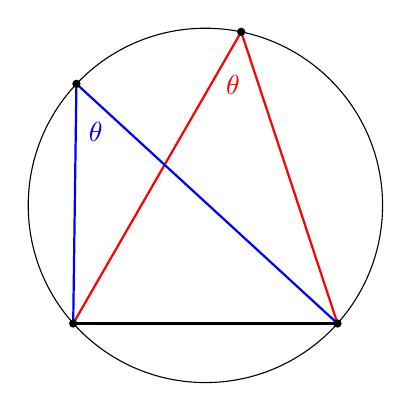
\begin{tikzpicture}[scale=.75]
% Circle goes from (a) to (b)
\coordinate (a) at (0,0);
\coordinate (b) at (6,0);
% Line containing lower points is (c) -- (d)
\coordinate (c) at (0,-2);
\coordinate (d) at (6,-2);
% Line containing upper points is (e) -- (f);
\coordinate (e) at (0,1.8);
\coordinate (f) at (3.8,3);
% Name the upper and lower lines
\path [name path=chord1] (c) -- (d);
\path [name path=chord2] (e) -- (f);
% Draw a circle whose center is half-way between (a) and (b) through (a)
\node [draw,circle through=(a),name path=circ] at ($ (a)!.5!(b) $) {};
% Get intersections of the upper and lower lines with the circle
\path [name intersections={of=circ and chord1,by={i1,i2}}];
\path [name intersections={of=circ and chord2,by={i3,i4}}];
% Draw the lower chord
\draw[thick] (i1) -- (i2);
% Draw the two subtended angles
\draw[thick,red] (i1) -- (i3)
  node[below,xshift=-3pt,yshift=-12pt] {$\theta$} -- (i2);
\draw[thick,blue] (i1) -- (i4)
  node[below,xshift=7pt,yshift=-10pt] {$\theta$} -- (i2);
% Dots at intersections
\fill (i1) circle (2pt);
\fill (i2) circle (2pt);
\fill (i3) circle (2pt);
\fill (i4) circle (2pt);
\end{tikzpicture}

% Thale's theorem 1
%
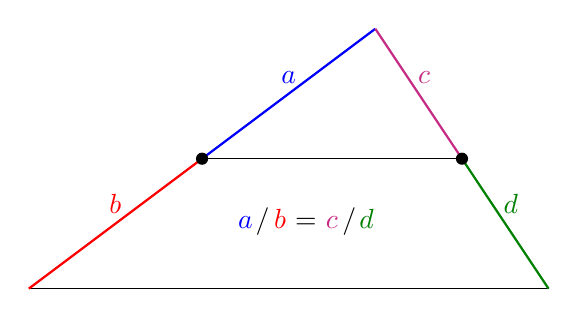
\begin{tikzpicture}[scale=1.1]
% Points of the triangle
\coordinate (a) at (0,0);
\coordinate (b) at (6,0);
\coordinate (c) at (4,3);
% Midpoints of the sides
\coordinate (mid1) at ($(a)!.5!(c)$);
\coordinate (mid2) at ($(b)!.5!(c)$);
\draw (a) -- (b);
% Draw the base and median
\draw (mid1) -- (mid2);
% Get the median
\coordinate (midbase) at ($(a)!.5!(b)$);
% Draw the triangle, sides in two parts
\draw[thick,red] (a) -- node[above] {$b$} (mid1);
\draw[thick,blue] (mid1) -- node[above] {$a$} (c);
\draw[thick,green!50!black] (b) -- node[above,xshift=2pt] {$d$} (mid2);
\draw[thick,magenta!80!black] (mid2) -- node[above,xshift=2pt] {$c$} (c);
% Dots at the midpoints
\fill (mid1) circle (2pt);
\fill (mid2) circle (2pt);
% Display formula in color
\begin{scope}[xshift=2.5cm,yshift=.7cm]
\node[anchor=base,blue] at (0,0) {$a$};
\node[anchor=base] at (.2,0) {$/$};
\node[anchor=base,red] at (.4,0) {$b$};
\node[anchor=base] at (.7,0) {$=$};
\node[anchor=base,magenta!80!black] at (1,0) {$c$};
\node[anchor=base] at (1.2,0) {$/$};
\node[anchor=base,green!50!black] at (1.4,0) {$d$};
\end{scope}
\end{tikzpicture}
